\documentclass[tikz,border=5pt]{standalone}
\usepackage{amssymb,amsmath}
\begin{document}
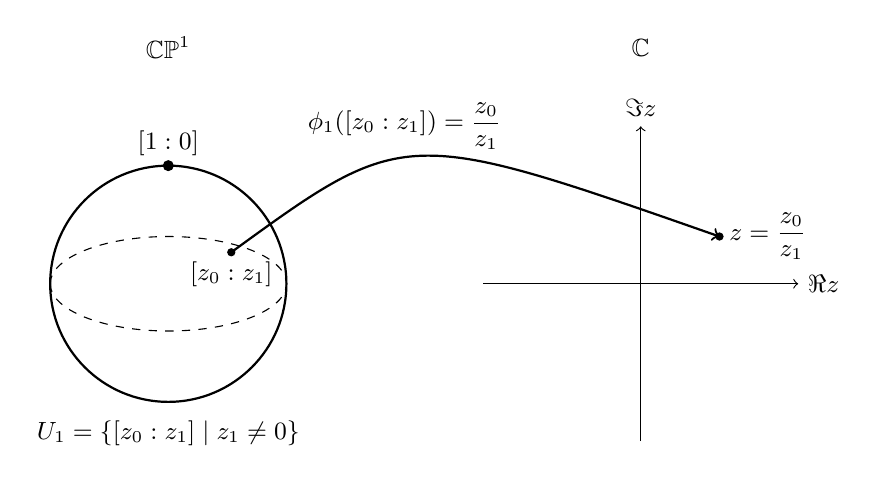
\begin{tikzpicture}[font=\small]
%----------------------------
% Left: CP^1 as a sphere
%----------------------------
\begin{scope}[shift={(-3,0)}]
	% Sphere (just a circle in 2D)
	\draw[thick] (0,0) circle (1.5);
	\node at (0,3) {$\mathbb{CP}^1$};
	
	% North pole = point at infinity [1:0]
	\fill (0,1.5) circle (2pt)
	node[above] {$[1:0]$};
	
	% Equator (to suggest the affine chart)
	\draw[dashed] (-1.5,0) arc (180:360:1.5 and 0.6);
	\draw[dashed] (-1.5,0) arc (180:0:1.5 and 0.6);
	
	% Label for U_1 (sphere minus the north pole)
	\node at (0,-1.9) {$U_1=\{[z_0:z_1]\mid z_1\neq 0\}$};
	
	% A generic point in U_1
	\fill (0.8,0.4) circle (1.5pt)
	node[below] {$[z_0:z_1]$};
\end{scope}

%----------------------------
% Right: Complex plane
%----------------------------
\begin{scope}[shift={(3,0)}]
	% Axes
	\draw[->] (-2,0)--(2,0) node[right] {$\Re z$};
	\draw[->] (0,-2)--(0,2) node[above] {$\Im z$};
	\node at (0,3) {$\mathbb{C}$};
	
	% Image point z = z0/z1
	\fill (1,0.6) circle (1.5pt);
	\node[right] at (1,0.6) {$z=\dfrac{z_0}{z_1}$};
\end{scope}

%----------------------------
% Arrow: phi_1
%----------------------------
% Global coordinates of the domain point: (-3+0.8, 0.4) = (-2.2, 0.4)
% Global coordinates of the image point: (3+1, 0.6) = (4, 0.6)
\draw[->,thick] (-2.2,0.4) .. controls (0,2) .. (4,0.6);
\node[] at (0,2) {$\phi_1([z_0:z_1])=\dfrac{z_0}{z_1}$};

\end{tikzpicture}
\end{document}
